\documentclass[12pt]{article}
\usepackage{times} 			% use Times New Roman font

\usepackage[margin=1in]{geometry}   % sets 1 inch margins on all sides
\usepackage{hyperref}               % for URL formatting
\usepackage[pdftex]{graphicx}       % So includegraphics will work
\setlength{\parskip}{1em}           % skip 1em between paragraphs
\usepackage{indentfirst}            % indent the first line of each paragraph
\usepackage{datetime}
\usepackage[small, bf]{caption}
\usepackage{listings}               % for code listings
\usepackage{xcolor}                 % for styling code
\usepackage{multirow}
\usepackage{xurl} 
\usepackage{enumitem}
\usepackage[section]{placeins}
\usepackage{float}
\usepackage{hyperref}
\usepackage{rotating}
\usepackage{tikz}

%New colors defined below
\definecolor{backcolour}{RGB}{246, 246, 246}   % 0xF6, 0xF6, 0xF6
\definecolor{codegreen}{RGB}{16, 124, 2}       % 0x10, 0x7C, 0x02
\definecolor{codepurple}{RGB}{170, 0, 217}     % 0xAA, 0x00, 0xD9
\definecolor{codered}{RGB}{154, 0, 18}         % 0x9A, 0x00, 0x12

%Code listing style named "gcolabstyle" - matches Google Colab
\lstdefinestyle{gcolabstyle}{
  basicstyle=\ttfamily\small,
  backgroundcolor=\color{backcolour},   
  commentstyle=\itshape\color{codegreen},
  keywordstyle=\color{codepurple},
  stringstyle=\color{codered},
  numberstyle=\ttfamily\footnotesize\color{darkgray}, 
  breakatwhitespace=false,         
  breaklines=true,                 
  captionpos=b,                    
  keepspaces=true,                 
  numbers=left,                    
  numbersep=5pt,                  
  showspaces=false,                
  showstringspaces=false,
  showtabs=false,                  
  tabsize=2
}

\lstset{style=gcolabstyle}      %set gcolabstyle code listing

\makeatletter
\g@addto@macro{\UrlBreaks}{\UrlOrds}
\makeatother

% for fancy page headings
\usepackage{fancyhdr}
\setlength{\headheight}{13.6pt} % to remove fancyhdr warning
\pagestyle{fancy}
\fancyhf{}
\rhead{\small \thepage}
\lhead{\small HW6, Lewis}  
\chead{\small CS 432, Fall 2020} 

%-------------------------------------------------------------------------
\begin{document}

\begin{centering}
{\large\textbf{HW6 - Analyzing Disinformation Domains}}

Brenden Lewis\\                     
Due: 11/15/2020 11:59PM\\                      
\end{centering}

%-------------------------------------------------------------------------
\section*{Q1}

Listing 1 below shows the code used to read in and process the D2 dataset. I decided it would be easiest to collect and process all URIs first before extracting and identifying unique domains. I used the \emph{requests} library to get the HTTP status code and final uri for each URI in the dataset; this processing was handled in the \emph{processHTTPStatus()} method that takes a URI as an argument.

\lstinputlisting[language=Python, caption=Python code for Q1, label=lst:import]{q1.py}

Once a URi was finished processing, a dictionary was created storing the original URI, its frequency in Twitter posts, final URI, and status code returned from \emph{requests.get}. An example of this structure is shown in Listing 2 below. Each dictionary per URI was stored in ProcessingURIs.txt; this allowed me to more easily test other code without having to re-process the URIs as it is a lengthy process at about 2 hours.

\begin{lstlisting}[language=Python, caption={Entry from ProcessedURIs.txt}, label=lst:copy]
{'OG_URI': 'http://newsteller.org', 'FREQUENCY': '2', 'FINAL_URI': 'http://newsteller.org/', 'STATUS': 200}
\end{lstlisting}

I utilized \emph{urlparse(uri).netloc} to extract the domain of a given uri. With the extracted domain and the passed in tweet frequency, I was created and stored dictionaries containing the domain, the number of times it appeared within the dataset, and tweet frequency in a dictionary list. Before they could be stored, however, I had to check first if the domain was already present in the list; if the domain was already present, the \emph{NUM\textunderscore IN\textunderscore DATA} value would need to be iterated by one. This was done simply by enumerating the list and using an index to access the domain and its values directly.

\par Listing 3 below shows the statistics for URI processing. Out of a total of 1679 URIs, 1186 resulted in a 200 status code while 493 resulted in a status code other than 200 (almost entirely 404, but there were one or two alternate codes). 793 of the URIs were redirected to a different URI.

\begin{lstlisting}[language=Python, caption={Stats from URI processing}, label=lst:copy]
URIs with 200 response: 1186
URIs with 404 response: 493
URIs redirected to different URIs: 793

Unique Domains: 812
\end{lstlisting}

Listing 4 shows a snippet of the unique domains sorted by their frequency in the data set. There were a total of 812 unique domains out of the 1679 URIs processed. Each listing shows the domain, its frequency in the data set, and the number of tweets they were featured in. Interestingly enough, among the most common domains in the data set were Google domains, with \emph{news.google.com} being the most prominent.

\par However, Google did not appear in the most amount of tweets in the set. Listing 5 shows the top 5 domains with the largest presence in twitter posts. Of the top listed domains, there are conspiracy theory sites, a US news outlet, a British newspaper, and a Middle Eastern news outlet. The domain that appeared in the most tweets was \emph{unz.com} with 514 tweets. The domain refers to an alternative media news outlet, discovered to be pushing conspiracy theories, anti-semitism, and whitee supremacy.

\begin{lstlisting}[language=Python, caption={Segment of unique domains sorted by frequency in data set}, label=lst:copy]
Number of Unique Domains: 812/1679 URIs

Domain: news.google.com
Frequency in Data: 40
Frequency in Twitter Posts: 1

Domain: www.newslocker.com
Frequency in Data: 38
Frequency in Twitter Posts: 1

Domain: 21stcenturywire.com
Frequency in Data: 36
Frequency in Twitter Posts: 29

Domain: www.google.com
Frequency in Data: 28
Frequency in Twitter Posts: 1

Domain: news.quiboat.com
Frequency in Data: 22
Frequency in Twitter Posts: 1

Domain: clarityofsignal.com
Frequency in Data: 20
Frequency in Twitter Posts: 464
\end{lstlisting}

From the data set, the top 5 domains that appeared in the most tweets were:
\begin{lstlisting}[language=Python, caption={Top 5 domains with most tweets}, label=lst:copy]
1. unz.com [514]
2. clarityofsignal.com [464]
3. nbcnews.com [316]
4. middleeasteye.net [279]
5. theguardian.com [242]
\end{lstlisting}

\section*{Q2}

Listing 6 shows the code used for Q2. To keep everything simple, I read in each data set and stored each item as a dictionary in seperate lists. To compare each data set, I used a set of nested for-loops (one for each data set) to compare the stored domains; because I forgot to do so in Q1, I had to use a regular expression to remove the "www." present in some domains in D2, and lower case the domains in D3 for even comparison. If any domains were equal across the data sets, they were add to a list of domains for the respective data set pairing. To ensure no duplicates, an additional check to the list was used to check if the domain was already present in the list.

\lstinputlisting[language=Python, caption=Python code for Q2, label=lst:import]{q2.py}

Listings 7-9 below show tables of each set-comparison with all the common domains. Listing 10 shows a comparison table between all data sets with the domains present all three. Interesting to note, the top domains across all domains nearly matches the top domains between every other comparison. Additionally, nearly all the common domains are conspiracy theory sites.

\begin{lstlisting}[language=Python, caption={Domains present in both D1 and D2}, label=lst:copy]
                            D1 & 2
0              21stcenturywire.com
1               abovetopsecret.com
2                 activistpost.com
3                beforeitsnews.com
4              blacklistednews.com
5                    breitbart.com
6                      cbsnews.com
7                          cnn.com
8                  dailymail.co.uk
9                dcclothesline.com
10        fellowshipoftheminds.com
11                     foxnews.com
12  fuhrerious88blog.wordpress.com
13               globalresearch.ca
14                       heavy.com
15                    infowars.com
16                  intellihub.com
17         investmentwatchblog.com
18      landdestroyer.blogspot.com
19                 lewrockwell.com
20                    mirror.co.uk
21                     nbcnews.com
22                    news.sky.com
23                 nydailynews.com
24                     nytimes.com
25                     presstv.com
26                          rt.com
27                 sputniknews.com
28                theantimedia.org
29               thedailybeast.com
30             thedailysheeple.com
31           theeventchronicle.com
32       thefreethoughtproject.com
33                 theguardian.com
34                theintercept.com
35         themillenniumreport.com
36               therussophile.org
37                     thestar.com
38            thetruthseeker.co.uk
39                         upi.com
40               veteranstoday.com
41              washingtonpost.com
42                   worldtruth.tv
43                yournewswire.com
\end{lstlisting}

\begin{lstlisting}[language=Python, caption={Domains present in both D2 and D3}, label=lst:copy]
                       D2 & 3
0         21stcenturywire.com
1            activistpost.com
2           beforeitsnews.com
3               breitbart.com
4    collective-evolution.com
5               davidicke.com
6           dcclothesline.com
7          de.sputniknews.com
8              deutsch.rt.com
9          fr.sputniknews.com
10           gellerreport.com
11          globalresearch.ca
12          humansarefree.com
13               infowars.com
14             intellihub.com
15           off-guardian.org
16                presstv.com
17       ronpaulinstitute.org
18               rubikon.news
19                   sott.net
20               theduran.com
21  thewashingtonstandard.com
22               ukcolumn.org
23              worldtruth.tv
\end{lstlisting}

\begin{lstlisting}[language=Python, caption={Domains present in both D1 and D3}, label=lst:copy]
                 D1 & 3
0   21stcenturywire.com
1      activistpost.com
2     beforeitsnews.com
3         breitbart.com
4     dcclothesline.com
5     globalresearch.ca
6          infowars.com
7        intellihub.com
8           presstv.com
9       wakingtimes.com
10        worldtruth.tv
11        zerohedge.com
\end{lstlisting}

\begin{lstlisting}[language=Python, caption={Domains present in all data sets}, label=lst:copy]
                In All
0  21stcenturywire.com
1     activistpost.com
2    beforeitsnews.com
3        breitbart.com
4    dcclothesline.com
5    globalresearch.ca
6         infowars.com
7       intellihub.com
8          presstv.com
9        worldtruth.tv
\end{lstlisting}

\section*{Q3}

I opted to use two different Python scripts to handle Q3: one to gather the tweets featuring domain links common between the D2 and D3 data set (Listing 11), and one to analyze the gathered tweets and create the appropriate graphs (Listing 13). 

\par For gathering tweets, I used Tweepy. For the sake of time, I limited the number of tweets per domain to a maximum of 200 tweets. At the same time, I filtered out any retweets using \emph{"-filter:retweets"} in the Cursor call. Each tweet was stored as a dictionary with its ID, the account that sent the tweet, the time it was tweeted, the domain featured in the tweet, the link to said domain as it appears in the text, and the full text in the tweet. 

\lstinputlisting[language=Python, caption=Python code for gathering tweets for Q3, label=lst:import]{gatherTweets.py}

Each captured tweet was exported to a JSON file called \emph{tweets.json}. The JSON format of each tweet in the file is shown below in Listing 12. This file is processed in \emph{q3.py}.

\begin{lstlisting}[language=Python, caption={Example tweet gathered in JSON}, label=lst:copy]
  {
    "ID": "1333480504297988104",
    "ACCOUNT": "Marie61172377",
    "TIME": "20201130183821",
    "DOMAIN": "21stcenturywire.com",
    "LINK": "https://21stcenturywire.com/2020/11/23/covid-19-mounting-evidence-of-international-fraud/",
    "TEXT_BODY": "COVID 19: Mounting Evidence of International Fraud - 21st Century Wire https://t.co/t6SPl6F6C5"
  }
\end{lstlisting}

The code for processing the \emph{tweets.json}, gathering tweet and domain statistics, and drawing graphs is featured below in Listing 13. Loading the data from \emph{tweets.json}, the data was passed into seperate functions to gather the different stats for Q3. 


\lstinputlisting[language=Python, caption=Python code for analyzing gathered tweets and drawing the graph for Q3, label=lst:import]{q3.py}

\par \emph{buildDomainStats()} was used to gather the number of tweets and accounts for each domain. A separate, temporary list of accounts was used for comparisons to ensure multiple tweets from a single account were not being accounted for when finding total account numbers.

\par \emph{findTimeRange()} was used to find the window of time of which all tweets gathered were posted. A list was used to contain the time for each tweet, and the \emph{min()} and \emph{max()} functions were used with the list as a parameter to get both the oldest and most recent times across the data. These two values were stored in a separate array for use in output.

\par The final stats are shown below in Listing 14. Each domain is listed with the number of tweets featuring that domain and the number of different accounts posting those tweets. Across all domains, there was a grand total of 2908 tweets gathered, with a collective number of 1156 different accounts that posted those tweets. The range of time across those tweets was November 21, 2020 12:25PM to November 30, 2020 7:29PM.

\begin{lstlisting}[language=Python, caption={Domain tweet and account statistics}, label=lst:copy]
Domain: 21stcenturywire.com
Number of Tweets: 207    
Number of Accounts: 88   


Domain: activistpost.com 
Number of Tweets: 204    
Number of Accounts: 79   


Domain: beforeitsnews.com
Number of Tweets: 69     
Number of Accounts: 33   


Domain: breitbart.com
Number of Tweets: 210
Number of Accounts: 122


Domain: collective-evolution.com
Number of Tweets: 205
Number of Accounts: 123


Domain: davidicke.com
Number of Tweets: 71
Number of Accounts: 52


Domain: dcclothesline.com
Number of Tweets: 202
Number of Accounts: 105


Domain: de.sputniknews.com
Number of Tweets: 5
Number of Accounts: 4


Domain: deutsch.rt.com
Number of Tweets: 14
Number of Accounts: 10


Domain: fr.sputniknews.com
Number of Tweets: 12
Number of Accounts: 11


Domain: gellerreport.com
Number of Tweets: 204
Number of Accounts: 81


Domain: globalresearch.ca
Number of Tweets: 0
Number of Accounts: 0


Domain: humansarefree.com
Number of Tweets: 207
Number of Accounts: 88


Domain: infowars.com
Number of Tweets: 231
Number of Accounts: 110


Domain: intellihub.com
Number of Tweets: 76
Number of Accounts: 28


Domain: off-guardian.org
Number of Tweets: 0
Number of Accounts: 0


Domain: presstv.com
Number of Tweets: 211
Number of Accounts: 64


Domain: ronpaulinstitute.org
Number of Tweets: 158
Number of Accounts: 81


Domain: rubikon.news
Number of Tweets: 10
Number of Accounts: 7


Domain: sott.net
Number of Tweets: 0
Number of Accounts: 0


Domain: theduran.com
Number of Tweets: 0
Number of Accounts: 0


Domain: thewashingtonstandard.com
Number of Tweets: 200
Number of Accounts: 30


Domain: ukcolumn.org
Number of Tweets: 207
Number of Accounts: 83


Domain: worldtruth.tv
Number of Tweets: 205
Number of Accounts: 28


Total Number of Tweets: 2908
Total Number of Accounts: 1156
Time Range: {20201121122509 --- 20201130192909} 
            #11/21/2020 12:25PM --- 11/30/2020 7:29PM
\end{lstlisting}

Figure 1 below shows a horizonantal bar chart visualizing the tweet counts for each domain, with the domains on the y-axis and tweet counts on the x-axis. Figure 2 shows the same domains with their account counts; these were drawn using the \emph{seaborn} visualization library. Unfortunantly, I was forced to rotate and scale them down to cleanly fit them in this report.

\begin{sidewaysfigure}
    \centering
    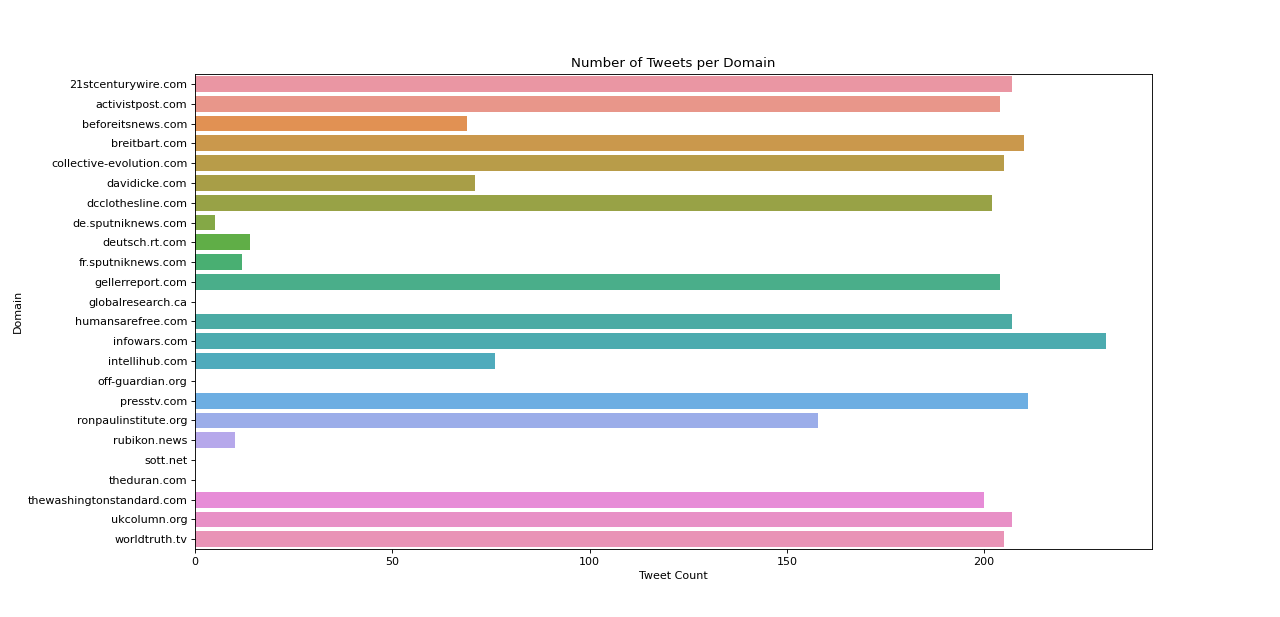
\includegraphics[scale = .58, trim = 10 17 0 30, clip]{DomainGraph.png}
    \caption{Graph showing the number of tweets per domain}
    \label{fig:my_label}
\end{sidewaysfigure}

\begin{sidewaysfigure}
    \centering
    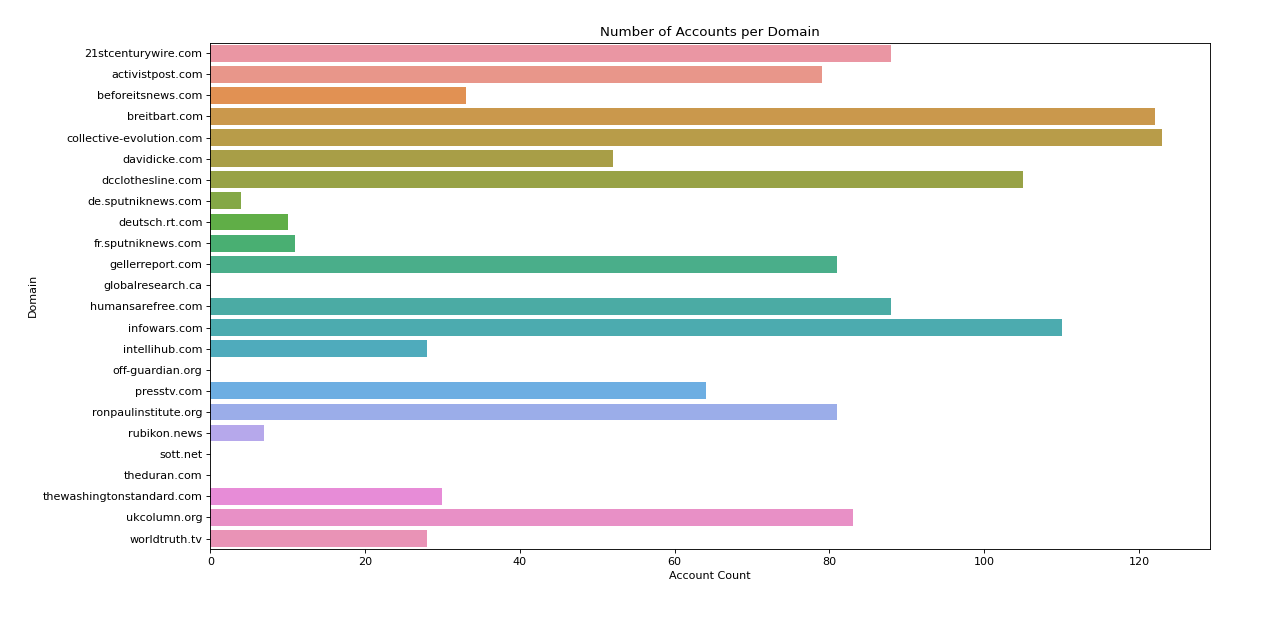
\includegraphics[scale = .58, trim = 10 17 0 20, clip]{DomainGraphAccounts.png}
    \caption{Graph showing the number of accounts per domain}
    \label{fig:my_label}
\end{sidewaysfigure}

\section*{Q4}

Listing 15 below features the code used for Q4. It is very similar in structure to the code in Q2, with the biggest differences being the replacement of the D3 data set with the data collected in Q3 (labeled Q3) and the comparison logic. Since there was no need to observe overlap in all three data sets, I used two seperate, nested for-loops for the comparisons between Q3 and D1/D2.

\lstinputlisting[language=Python, caption=Python code for Q4, label=lst:import]{q4.py}

Listing 16 below shows the top 5 common domains for each comparison set and the number of times they were featured in each individual data set. These were found by counting the total number of tweets a domain was featured in between each data set. 

\par Based on the results, there were a few domains that shared a top 5 spot in each comparison, namely \emph{dcclothesline.com} and \emph{activistpost.com}. These two had a much larger presence in the D1 data set than the D2 data set. Of note, there is much larger disparity between the tweet counts in the \emph{D1\textunderscore Q3} distribution than in the \emph{D2\textunderscore Q3} distribution. \emph{infowars.com} in particular heavily skews the distrbution with its presence in the D1 data.

\begin{lstlisting}[language=Python, caption={Top 5 domains per data set comparison}, label=lst:copy]
Top 5 Shared Domains in Set D1_Q3:

Domain: infowars.com
Total Tweet Count from Domain in Set: 1972
Tweet Count from D1: 1741
Tweet Count from Q3: 231

Domain: beforeitsnews.com
Total Tweet Count from Domain in Set: 649
Tweet Count from D1: 580
Tweet Count from Q3: 69

Domain: dcclothesline.com
Total Tweet Count from Domain in Set: 435
Tweet Count from D1: 233
Tweet Count from Q3: 202

Domain: activistpost.com
Total Tweet Count from Domain in Set: 379
Tweet Count from D1: 175
Tweet Count from Q3: 204

Domain: 21stcenturywire.com
Total Tweet Count from Domain in Set: 269
Tweet Count from D1: 62
Tweet Count from Q3: 207

----------------------------------------

Top 5 Shared Domains in Set D2_Q3:

Domain: gellerreport.com
Total Tweet Count from Domain in Set: 438
Tweet Count from D2: 234
Tweet Count from Q3: 204

Domain: dcclothesline.com
Total Tweet Count from Domain in Set: 298
Tweet Count from D2: 96
Tweet Count from Q3: 202

Domain: activistpost.com
Total Tweet Count from Domain in Set: 287
Tweet Count from D2: 83
Tweet Count from Q3: 204

Domain: collective-evolution.com
Total Tweet Count from Domain in Set: 255
Tweet Count from D2: 50
Tweet Count from Q3: 205

Domain: ronpaulinstitute.org
Total Tweet Count from Domain in Set: 250
Tweet Count from D2: 92
Tweet Count from Q3: 158
\end{lstlisting}

Figures 3 and 4 below show visualizations of the above data for each domain in each comparison.

\begin{figure}[H]
            \centering
            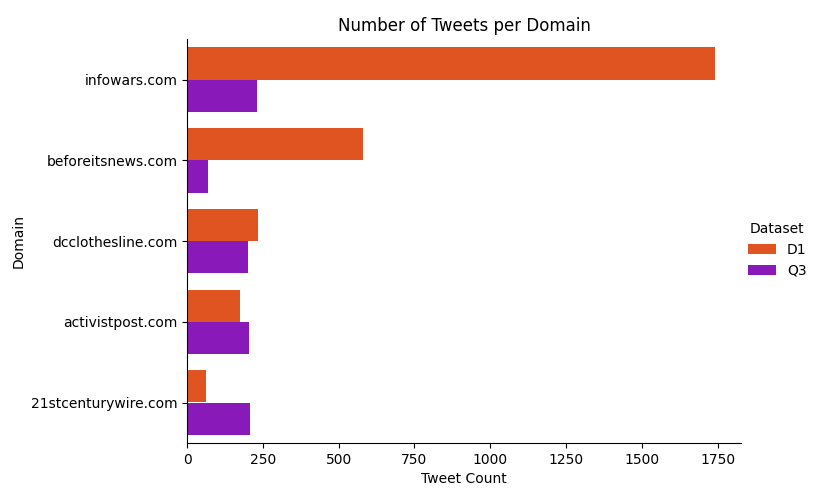
\includegraphics[scale=0.8,trim = 9 0 0 0, clip]{Q4_D1Q3_Graph.png}
            \caption{Top 5 domains shared between datasets D1 and Q3}
            \label{fig:my_label}
        \end{figure}
        
\begin{figure}[H]
            \centering
            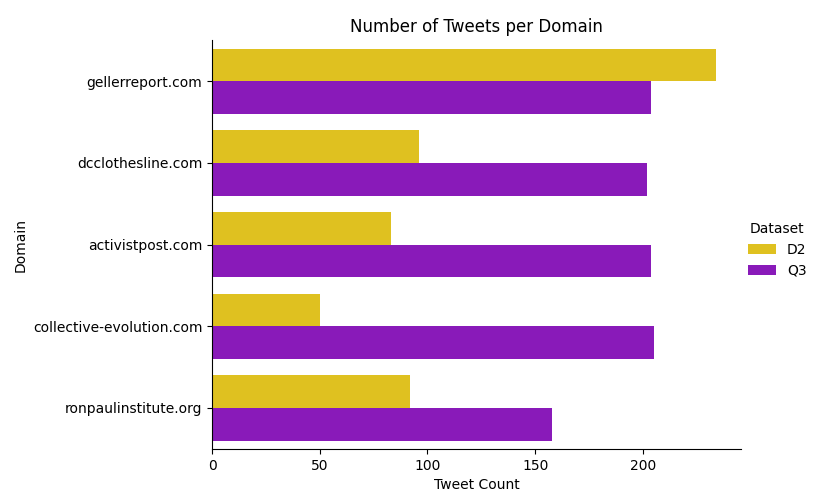
\includegraphics[scale=0.8,trim = 9 0 0 0, clip]{Q4_D2Q3_Graph.png}
            \caption{Top 5 domains shared between datasets D2 and Q3}
            \label{fig:my_label}
        \end{figure}

\section*{Q6 (Extra Credit)}

Listing 17 below features the code used for Q6. In order to properly analyze the text of the collected tweets, I needed to read in \emph{tweets.json} from Q3 and clean each tweet by removing all special characters, URI links, and stopwords from the text bodies to isolate the prominant words in each tweet. 

\par For each tweet, I passed the text into the \emph{removeUrlsAndSpecialChars()} method. This method used a regular expression to remove any non-Alpha characters from the text; the resulting string was also lowercased to help later with removing stopwords. The text was then split into a list to isolate each word, and then stored in another list (\emph{tweet\textunderscore Bodies}) containing each split text with the same index as the tweet it came from in the original data.

\par With the resulting list of lists, a nested for-loop was used to access each word in each text body. For each tweet body, a temporary list created, and each word was compared to a list of english stopwords provided by the Natural Language ToolKit (\emph{nltk}) library. If a word was not present in the stopword list (not a stopword), it was added to the temporary list, and the list was stored in a new list called \emph{tweets\textunderscore no\textunderscore stops}; this list is identical in structure to the previous (\emph{tweet\textunderscore Bodies}) minus the stopwords in each text body. To assist with additional analysis, a final string list was created to hold every word across all the cleaned text bodies.

\par I wanted to find the most common terms across all the gathered tweets to help highlight the overall topics discussed across them. In order to find the most common terms, I used some functions featured in the Counter class from the \emph{collections} library. In the \emph{getMostCommonTerms()} method, I created a Counter object from \emph{all\textunderscore words} and used \emph{most\textunderscore common(20)} to get the top 20 most common words and the number of times they appeared (somehow the resulting top two words were stopwords that slipped through cleaning, so I had to get the top 22 words and remove the first two). The words and their counts are returned as individual lists that I stored in \emph{most\textunderscore common}. I also created a seperate list specifically to hold only the words called \emph{common}.

\par With the common terms found, I ran a check across all tweets to see which tweets contained any of the common terms; this was handled in the \emph{checkCommonTerms()} method. Going through each split body of text and each common term in a nested loop, a counter was incremented if a common word was present within the text. Since I was only checking if a tweet contained any of the common terms, the boolean \emph{breaker} was used to break from the loop if a common term was found.

\lstinputlisting[language=Python, caption=Python code for Q6, label=lst:import]{q6.py}

Listing 18 below shows the common terms, how many times they appeared in the data, and the number of tweets featuring a common term. Of the collected tweets, 1468 featured one of these common terms in their text bodies. Considering the time window of the tweets from Q3, these tweets were posted in the few weeks following the US election. Even without knowing the time window, the large majority of the common terms are all buzzwords used in relation to the US election results, the widespread claims of voter fraud, and the COVID-19 pandemic. 

\par Voter fraud in regards to the 2020 election is a very topical subject, and while these claims have been shot down in every court case due to lack of evidence, misinformation about the election results still continues to circulate and garner a lot of attention. In this context, it makes sense that these terms would be common amongst domains that aim to spread misinformation. 

\par An interesting thing to note, however, is that the actual top term is \emph{election}, as \emph{worldtruthtv} is derived from the domain \emph{worldtruth.tv} (it somehow made it past the link-removal in cleanup). However, I was curious so I looked into it, and it is a literal fake news website; it is even labeled as an "alternative news network" on the site. It's clear based on the article content and how they're worded that the site is pushing out false information based on conspiracy theories. It is slightly disturbing how a site like this and its content can be spread around so easily on social media platforms like Twitter. 

\begin{lstlisting}[language=Python, caption={Most common terms across gathered tweets, ordered by number of tweets they appeared in}, label=lst:copy]
Top 20 most common terms out of 2908 Tweets

('worldtruthtv', 163)
('election', 161)
('trump', 141)
('covid19', 135)
('us', 132)
('state', 128)
('covid', 124)
('cia', 123)
('new', 119)
('people', 113)
('fraud', 111)
('news', 101)
('update', 97)
('war', 94)
('breitbartnews', 93)
('uk', 90)
('dominion', 87)
('says', 87)
('situation', 85)
('vaccine', 84)

Number of Tweets featuring a common term: 1468
\end{lstlisting}

\end{document}
